% copyright (c) 2018 Groupoid Infinity

\documentclass{svproc}
\usepackage{amscd}
\usepackage{listings}
\usepackage[numbers]{natbib}
\usepackage[only,llbracket,rrbracket,llparenthesis,rrparenthesis]{stmaryrd}
\usepackage{graphicx}
\usepackage{amsmath}
\usepackage{amssymb}
\usepackage{txfonts}
\usepackage[utf8]{inputenc}
\usepackage[numbers]{natbib}

\renewcommand\bibsection{\section*{\refname}\small\renewcommand\bibnumfmt[1]{##1.}}
\lstset{basicstyle=\small,inputencoding=utf8}

\begin{document}

\title{Constructive Proofs \\
       of Heterogeneous Equalities \\
       in Cubical Type Theory}
\author{Maksym Sokhatskyi $^1$ and Pavlo Maslianko $^1$}
\date{
    $^1$ National Technical University of Ukraine \\
    \small Igor Sikorsky Kyiv Polytechnical Institute\\
    \today
}

\maketitle

\begin{abstract}
This paper represents the very small part of the developed base library for homotopical
prover based on Cubical Type Theory (CTT) announced in 2017. We demonstrate the usage
of this library by showing how to build a constructive proof of heterogeneous equality,
the simple and elegant formulation of the equality problem, that was impossible to achieve
in pure Martin-Löf Type Theory (MLTT). The machinery used in this article unveils
the internal aspect of path equalities and isomorphism, used e.g. for proving univalence
axiom, that became possible only in CTT. As an example of complex proof that was
impossible to construct in earlier theories we took isomorphism between Nat and Fix Maybe
datatypes and built a constructive proof of equality between elements of these datatypes.
This approach could be extended to any complex isomorphic data types.
\end{abstract}

{\bf Keywords}: Formal Methods, Type Theory, Computer Languages,
          Theoretical Computer Science, Applied Mathematics,
          Isomorphism, Heterogeneous Equality, Cubical Type Theory,
          Martin-Löf Type Theory

%\newpage
%\tableofcontents
%\newpage

\section{Intro}

After formulating Type Theory to model quantifiers using $Pi$ and $Sigma$ types in 1972 \cite{Lof72}
Per Martin-Löf added $Equ$ equality types in 1984 \cite{Lof84}. Later $Equ$ types were extended
to non-trivial structural higher equalities ($\infty$-groupoid model) as was shown by Martin Hofmann
and Thomas Streicher in 1996 \cite{Hofmann96}. However formal constructing of Equ type
eliminators was made possible only after introducing Cubical Type Theory in 2017 \cite{Mortberg17}.
CTT extends MLTT with interval $I=[0,1]$ and its de Morgan algebra: $0, 1, r, -r, min(r,s), max(r,s)$
allowing constructive proofs of earlier models based on groupoid interpretation.

{\bf The problem and tools used}. In this paper, we want to present the constructive formulation of proof
that two values of different types are equal using constructive heterogeneous equality
in Cubical Type Checker \cite{Mortberg17} \footnote{https://github.com/mortberg/cubicaltt}.
In the end, we will use path isomorphism for that purposes \cite{HoTT}.

{\bf Author's contribution}. During the story of comparing two zeros,
we will show the minimal set of primitives needed
for performing this task in the cubical type checker. Most of
them were impossible to derive in pure MLTT. We show these primitives in dependency order
while constructing our proof. This article covers different topics in type theory,
which is the main motivation to show how powerful the notion of equality is:
1) Complete Formal Specification of MLTT;
2) Contractability and n-Groupoids;
3) Constructive J;
4) Functional Extensionality;
5) Fibers and Equivalence;
6) Isomorphism;
7) Heterogeneous equality.

\subsection{Research Formal Description}

As a formal description of the research includes all cubical programs as research object,
type theory ingenral and MLTT and CTT inparticular as research subject,
direct proof construction as logical method and encoded cubical
base library and examples as research results.

{\bf Research object}. The homotopy type theory base libraries in Agda, Cubical, Lean and Coq.
While modern Agda has the cubical mode, Coq lacks of the computational semantics of path primitives
while has HoTT library. The real programming language is not enough to
develop the software and theorems, the language shoud be shipped with base library. In this article
we unvail the practical implementation of base library for cubical typecheckers.

{\bf Research subject}. We will analyze the base library through the needs of particular features,
like basic theorems, heterogeneous path equalities, univalence, basic HITs like truncations, run-time
versions of the list, nat, and stream datatypes. We use Martin-Löf Type Theory as a subject and
its extention CTT. The main motivation is to have small and concise base library for cubicaltt
type checker than can be used in more complex proofs. As an example of library usage we will show
the general sketch of the constructive proofs of heterogeneous equality in CTT, concentrating only
on homotopical features of CTT.

{\bf Research results}. Research result is presented as source code repository that can be used by
cubicaltt \footnote{http://github.com/mortberg/cubicaltt} language and contains the minimal base library used in this article.
These primitives form a valuable part of base library, so this arcticle could be
considered as an brief introduction to several modules: {\bf proto\_path}, {\bf proto\_equiv}, {\bf pi},
{\bf sigma}, {\bf mltt}, {\bf path}, {\bf iso}. But the library has even more modules, that
exceed the scope of this article so you may refer to source code
repository\footnote{http://github.com/groupoid/infinity}. Brief list of base library modules is given
in Conclusion.

\begin{figure}[h]
  \centerline{\includegraphics[scale=0.36]{cutbase}}
  \caption{Base library and its dependencies used in article}
\end{figure}

{\bf Research methods}. The formal definition of MLTT theory and constructive
implementation of its instance that supplied with minimal but comprehensive base library that
can be used for verifying homotopical and run-time models. The type theory itself is a modeling
language, logical framework and research method. The MLTT is a particular type theory with
$Universes$, $\Pi$, $\Sigma$ and $Equ$ types. This is common denominator for a series of provers
based on MLTT such as Coq, Agda, Cubicaltt, Idris. In the article we will use Cubical language.

\section{MLTT Type Theory}

MLTT is considered as contemporary common math modeling language for different parts of mathematics.
Thanks to Vladimir Voevodsky this was extended to Homotopy Theory
using MLTT-based Coq proof assistant \footnote{http://github.com/UniMath}.
Also he formulated the univalence principle $Iso(A,B)=(A=B)$ \cite{HoTT},
however constructive proof that isomorphism equals to equality and equivalences is possible only
in Cubical Type Theory \cite{Mortberg17} (Agda and Cubical type checkers).

In this section we will briefly discribe the basic notion of MLTT, then will give a formal
description of MLTT and the informal primitives of CTT. Only after that will start
the proof of heterogeneous equality ended up with proofterm. MLTT consist of
$\Pi$, $\Sigma$ and $Equ$ types living in a Hierarchy of universes $U_i : U_{i+1}$. We will
also give an extended equality $HeteroEqu$ which is needed for our proof.

\subsection{Syntax Notes}

Types are the analogues of sets in ZFC, or objects in topos theory, or spaces in analisys.
Types contains elements, or points, or inhabitans and it's denoted $a : A$ and there
is definitional equality which usually built into type checker and compare normal forms.

\begin{equation}
\tag{terms and types}
a : A
\end{equation}

\begin{equation}
\tag{definitional equality}
x = [ y : A ]
\end{equation}

MLTT type theory with $Pi$ and $Sigma$ types was formulated using
natural deduction inference rules as a language.
The inference rules in that language will
be translated to cubicaltt in our article.

\begin{equation}
\tag{natural deduction}
\dfrac
{(A: U_i)\ (B: A \rightarrow U_j)}
{(x: A) \rightarrow B(x): U_{max(i,j)}}
\end{equation}
\\
Equvalent definition in cubicaltt (which is inconstend $U : U$ but
this won't affect correctness of our proof). Here we consider $\Pi$
and $Pi$ synonimically identical. 

\begin{equation}
\tag{cubicaltt}
Pi\ (A: U)\ (B: A \rightarrow U): U = (x: A) \rightarrow B(x)
\end{equation}

In article we will use the latter notation, the cubical syntax.
The function name in cubical syntax is an inference rule name,
everything from name to semicolon is context conditions,
and after semicolon is a new consruction derived from context conditions.
From semicolon to equality sign we have type and after
equ sign we have the term of that type.
If the types are treated as spaces then terms are points in these spaces.

According to MLTT each type has 4 sorts of inference rules:
Formation, Introduction, Eliminators and Computational rules.
Formation rules are formal definition of spaces while introduction rules
are methods how to create points in these spaces. Introduction rules increase term size,
while eliminators reduce term size. Computational rules always
formulated as equations that represents reduction rules,
or operational semantics.

\subsection{Pi types}

$Pi$ types represent spaces of dependent functions.
With $Pi$ type we have one lambda constructor
and one application eliminator. When $B$ is not dependent on $x:A$
the $Pi$ is just a non-dependent total function $A \rightarrow B$.
$Pi$ has one lambda function constructor, and its eliminator, the
application \cite{HoTT, Lof72, Lof84, Hofmann96, Mortberg17, Ulf09}.

$$Pi(A,B) = \prod_{x:A} B(x) : U,\ \ \ 
  \lambda x . b : \prod_{x:A} B(x)$$

$$\prod_{f:\prod_{x:A}B(x)}\prod_{a:A} f a : B (a)$$

Here we formulate the math formula of $Pi$ and its eliminators in cubical syntax as Pi.
Note that backslash "\textbackslash"\  in cubical syntax means $\lambda$ function from math notation
and has compatible lambda signature.

\begin{lstlisting}[mathescape=true]
Pi (A:U) (B:A->U) : U = (x:A)->B(x)
lambda (A:U) (B:A->U) (a:A) (b:B(a)): A->B(a) = \ (x:A)->b
app (A:U) (B:A->U) (a:A) (f:A->B(a)): B(a) = f(a)
\end{lstlisting}

\subsection{Sigma types}

$Sigma$ types represents a dependent cartesian products.
With sigma type we have pair constructor and two eliminators,
its first and second projections. When $B$ is not dependent on $x:A$
the $Sigma$ is just a non-dependent product $A \times B$.
$Sigma$ has one pair constructor and two eliminators, its projections
\cite{HoTT, Lof72, Lof84, Hofmann96, Mortberg17, Ulf09}.

$$Sigma(A,B) = \sum_{x:A} B(x) : U,\ \ \ 
  (a,b) : \sum_{x:A} B(x)$$

$$\pi_1 : \prod_{f:\sum_{x:A}B(x)}A\ ,\ \ \ \pi_2 : \prod_{f:\sum_{x:A}B(x)}B(\pi_1(f))$$

As $Pi$ and $Sigma$ are dual the $Sigma$ type could be formulated
in terms of $Pi$ type using Church encoding, thus $Sigma$ is optional.
The type systems which contains only $Pi$ types called Pure or PTS.
Here we rewrite the math formula of $Sigma$ and its eliminators in cubical syntax as Sigma:

\begin{lstlisting}[mathescape=true]
Sigma (A:U) (B:A->U): U = (x:A) * B(x)
pair (A:U) (B:A->U) (a: A) (b: B(a)): Sigma A B = (a,b)
pr1 (A:U) (B:A->U) (x: Sigma A B): A = x.1
pr2 (A:U) (B:A->U) (x: Sigma A B): B (pr1 A B x) = x.2
\end{lstlisting}

\subsection{Equ types}

For modeling propositional equality later in 1984 was introduced $Equ$ type. \cite{Lof84}
However unlike $Pi$ and $Sigma$ the eliminator J of $Equ$ type is
not derivable in MLTT \cite{Hofmann96, Mortberg17, HoTT}.

$$Equ(x,y) = \prod_{x,y:A} x =_A y : U,\ \ \ 
  reflect : \prod_{a:A} a =_A a$$
$$D : \prod_{x,y:A}^{A:U_i} x =_A y \rightarrow U_{i+1},\ \ \ 
  J : \prod_{C: D} \prod_{x:A} C(x,x,reflect(x)) \rightarrow \prod_{y:A} \prod_{p:x=_A y} C(x,y,p)$$

Eliminator of Equality has complex form and underivable in MLTT.
Here we can see the formulation of $Equ$ in cubical syntax as Equ:

\begin{lstlisting}[mathescape=true]
Equ     (A: U) (x y: A): U = undefined
reflect (A: U) (a: A): Equ A a a = undefined
D       (A: U) : U = (x y: A) -> Equ A x y -> U
J       (A: U) (x y: A) (C: D A) (d: C x x (reflect A x))
                     (p: Equ A x y): C x y p = undefined
\end{lstlisting}

Starting from MLTT until cubicaltt there was no computational semantics
for J rules and in Agda and Coq it was formulated using inductive data types
wrapper around built-in primitives (J) in the core:

\begin{lstlisting}[mathescape=true]
data Equality (A:U) (x y:A) = refl_ (_: Equ A x z)
reflection (A:U) (a:A): Equality A a a = refl_ (reflect A a)
\end{lstlisting}

Heterogeneous equality is needed for computational rule of $Equ$ type.
And also this is crucial to our main task, constructive
comparison of two values of different types. We leave the definition blank
until introdure cubical primitives, here is just MLTT signature of HeteroEqu
which is undervable in MLTT.

\begin{lstlisting}[mathescape=true]
HeteroEqu (A B:U)(a:A)(b:B)(P:Equ U A B):U = undefined
\end{lstlisting}

E.g. we can define Setoid specification \cite{Bishop67} as not-MLTT basis
for equality types. These signatures are also underivable in MLTT.

$$symm : \prod_{a,b:A} \prod_{p:a =_A b} b =_A a,\ \ \ 
  transitivity : \prod_{a,b,c: A} \prod_{p: a =_A b} \prod_{q: b =_A c} a =_A c$$

\begin{lstlisting}[mathescape=true]
sym  (A:U)(a b:A)(p:Equ A a b): Equ A b a = undefined
transitivity (A:U)(a b c:A)(p: Equ A a b)(q: Equ A b c):
             Equ A a c = undefined
\end{lstlisting}

\subsection{Complete Formal Specification of MLTT}

MLTT needn't and hasn't the underlying logic, the Logical Framework could be constructed directly in MLTT.
According to Brouwer-Heyting-Kolmogorov interpretation the propositions are types,
Pi is an universal quantifier, Sigma is existential quantifier.
Implication is given by Pi over types, conjunction is cartesian
product of tpes and disjunction is disjoint sum of types.

So we can build LF for MLTT inside MLTT. Specification could be formulated as a
single Sigma chain holding the computation system and its theorems in one package.
Carrying object along with its properties called type refinement, so this type
represents a refined MLTT:

\begin{lstlisting}[mathescape=true]
MLTT (A:U): U
  = (Pi_Former:  (A->U)->U)
  * (Pi_Intro:   (B:A->U) (a:A)->B a->(A->B a))
  * (Pi_Elim:    (B:A->U) (a:A)->(A->B a)->B a)
  * (Pi_Comp1:   (B:A->U) (a:A) (f:A->B a) -> Equ (B a)
                 (Pi_Elim B a (Pi_Intro B a (f a)))(f a))
  * (Pi_Comp2:   (B: A->U) (a:A) (f:A->B a) ->
                 Equ (A->B a) f (\(x:A)->Pi_Elim B a f))
  * (Sig_Former: (A->U)->U)
  * (Sig_Intro:  (B:A->U) (a:A)->(b:B a)->Sigma A B)
  * (Sig_Elim1:  (B:A->U)->(_: Sigma A B)->A)
  * (Sig_Elim2:  (B:A->U)->(x: Sigma A B)->B (pr1 A B x))
  * (Sig_Comp1:  (B:A->U) (a:A) (b: B a)->Equ A a
                 (Sigma_Elim1 B (Sigma_Intro B a b)))
  * (Sig_Comp2:  (B:A->U) (a:A) (b:B a)->Equ (B a) b
                 (Sigma_Elim2 B (a,b)))
  * (Id_Former:  A->A->U)
  * (Id_Intro:   (a:A) -> Equ A a a)
  * (Id_Elim:    (a x: A) (C: predicate A a)
                 (d:C a(Id_Intro a))(p:Equ A a x)->C x p)
  * (Id_Comp:    (x y:A)(C: D A)(p: Equ A x y)
                              (b: C x x (reflect A x))
                       (X: Equ U (C x x (reflect A x))
                                 (C x y p)) ->
                   HeteroEqu X b (J A x C b y p)) * Unit
\end{lstlisting}

Even more complex challanges on Equ type was introduced such
as heterogeneous equality $HeteroEqu$ needed to formulation
of computational rule $Id\_Comp$ of $Equ$ type. Presheaf model of Type Theory, specifically
Cubical Sets with interval $[0,1]$ and
its algebra was introduced to solve derivability issues. So the instance of MLTT is packed
with all the type inference rules along with operational semantics:

\begin{lstlisting}[mathescape=true]
instance (A: U): MLTT A
    = (Pi A, lambda A, app A, comp1 A, comp2 A,
       Sigma A, pair A, pr1 A, pr2 A, comp3 A, comp4 A,
       Equ A, reflect A, J A, comp5 A, tt)
\end{lstlisting}


\section{Preliminaries}

\subsection{Cubical Type Theory Primitives and Syntax}

The path equality is modeled as an interval [0,1] with
its de Morgan algebra 0, 1, r, min(r,s), max(r,s). According to underlying theory
it has lambdas, application, composition and gluening of [0,1] interval and Min and Max
functions over interval arguments. This is enought to formulate and prove path
isomorphism and heterogeneous equality.

{\bf Heterogeneous Path}. The HeteroPath formation rule defines a heterogenous path
between elements of two types A and B for which Path exists A = B.

{\bf Abstraction over [0,1]}. Path lambda abstraction is a function which is defined on $[0,1]$:
$f: [0,1] \rightarrow A$. Path lambda abstraction is an element of Path type.

{\bf Min, Max and Invert}. In the body of lambda abstraction besides path application
de Morgan operation also could be used: $i \wedge j$, $i \vee j$, $i$, $-i$ and constants $0$ and $1$.

{\bf Application of path to element of [0,1]}. When path lambda is defined, the path term
in the body of the function could be reduced using lambda parameter applied to path term.

{\bf Path composition}. The composition operation states that being extensible
is preserved along paths: if a path is extensible at 0, then it is extensible at 1.

{\bf Path gluening}. The path gluening is an operation that allows to build
path from equivalences. CTT distinguishes types gluening, value gluening and ungluening.

Here we give LALR specification of BNF notation of Cubicat Syntax as implemented
in our github repository \footnote{http://github.com/groupoid/infinity/}. It has
only 5 keywords: {\bf data}, {\bf split}, {\bf where}, {\bf module}, and {\bf import}.

\begin{lstlisting}[mathescape=true]
def := ${\bf data}$ id tele = sum + id tele : exp = exp +
       id tele : exp ${\bf where}$ def
exp := cotele*exp + cotele$\rightarrow$exp + exp$\rightarrow$exp + (exp) + app + id +
       (exp,exp) + \ cotele$\rightarrow$exp + ${\bf split}$ cobrs + exp${\bf.1}$ + exp${\bf.2}$
  0 := #empty         imp    := [ ${\bf import}$ id ]
brs := 0 + cobrs      tele   := 0 + cotele
app := exp exp        cotele := ( exp : exp ) tele
 id := [ #nat ]       sum    := 0 + id tele + id tele | sum
ids := [ id ]         br     := ids $\rightarrow$ exp
cod := def dec        mod    := ${\bf module}$ id ${\bf where}$ imp def
dec := 0 + codec      cobrs  := | br brs
\end{lstlisting}

\subsection{Contractability and Higher Equalities}

A type $A$ is contractible, or a singleton, if there is $a : A$,
called the center of contraction, such that $a = x$ for all $x : A$:
A type $A$ is proposition if any x,y: A are equals.
A type is a Set if all equalities in A form a prop.
It is defined as recursive definition.

$$isContr = \sum_{a:A}\prod_{x:A} a =_A x,\ \ 
  isProp(A) = \prod_{x,y:A} x =_A y,\ \ 
  isSet = \prod_{x,y:A} isProp\ (x =_A y),\ \ $$
$$isGroupoid = \prod_{x,y:A} isSet\ (x =_A y),\ \ 
  PROP = \sum_{X:U}isProp(X),\ \ 
  SET = \sum_{X:U}isSet(X),...$$

The following types are inhabited: isSet PROP, isGroupoid SET.
All these functions are defined in {\bf path} module. As you can see
from definition there is a recurrent pattern which we encode in cubical syntax
as follows:

\begin{lstlisting}[mathescape=true]
${\bf data}$ N = Z | S (n: N)
n_grpd (A: U) (n: N): U = (a b: A) -> ((rec A a b) n) where
  rec (A: U) (a b: A): (k: N) -> U = ${\bf split}$
    Z -> Path A a b
    S n -> n_grpd (Path A a b) n

isContr (A: U): U = (x:A) * ((y: A) -> Equ A x y)
isProp      (A: U): U = n_grpd A Z
isSet       (A: U): U = n_grpd A (S Z)
isGroupoid  (A: U): U = n_grpd A (S (S Z))
PROP      : U = (X:U) * isProp X
SET       : U = (X:U) * isSet  X
GRPOUPOID : U = (X:U) * isGroupoid X
\end{lstlisting}

\subsection{Constructive J}

The very basic ground of type checker is heterogeneous equality $PathP$ and contructive
implementation of reflection rule as lambda over interval $[0,1]$ that
return constant value $a$ on all domain.

\begin{lstlisting}[mathescape=true]
Path (A:U)(a b:A):U = PathP (<i>A) a b
HeteroEqu (A B:U)(a:A)(b:B)(P:Equ U A B):U = Path P a b
refl (A:U)(a:A):Path A a a = <i> a
sym (A:U)(a b:A) (p: Path A a b): Path A b a = <i> p @ -i
transitivity (A: U)(a b c:A)(p: Path A a b) (q: Path A b c):
    Path A a c = comp (<i> Path A a (q @ i)) p []
\end{lstlisting}

$$trans : \prod_{p:A=_U B}^{A,B:U} \prod_{a:A} B,\ \ \ singleton : \prod_{x:A}^{A:U} \sum_{y:A} x =_A y $$

$$subst : \prod_{a,b:A}^{A:U,B:A\rightarrow U} \prod_{p: a =_A b} \prod_{e:B(a)} B(b), \ \ \ 
  congruence : \prod_{f:A\rightarrow B}^{A,B:U} \prod_{a,b:A} \prod_{p:a =_A b} f(a) =_B f(b) $$

Transport tranfers the element of type to another by given path equality of the types.
Substitution is like transport but for dependent functions values: by given dependent function
and path equality of points in the function domain we can replace the value of dependent function
in one point with value in the second point. Congruence states that for a given function
and for any two points in the function domain, that are connected, we can state that function
values in that points are equal.

\begin{lstlisting}[mathescape=true]
singl (A:U) (a:A): U = (x: A) * Path A a x
trans (A B:U) (p: Path U A B) (a: A): B = comp p a []
congruence (A B: U) (f:A->B) (a b: A)
           (p: Path A a b): Path B (f a) (f b)
           = <i> f (p @ i)

subst (A:U) (P:A->U) (a b: A)
      (p: Path A a b) (e: P a): P b
      = trans (P a) (P b) (congruence A U P a b p) e

contrSingl (A : U) (a b : A) (p : Path A a b):
           Path (singl A a) (a,refl A a) (b,p)
           = <i> (p @ i, <j> p @ i /\ j )
\end{lstlisting}

Then we can derive J using $contrSingl$ and $subst$ as defined in HoTT\cite{HoTT}:

\begin{lstlisting}[mathescape=true]
J (A:U)(x y:A)(C: D A)(d:C x x (refl A x))
         (p:Path A x y): C x y p =
   subst (singl A x) T (x,refl A x)
         (y,p) (contrSingl A x y p) d where
       T (z:singl A x):U = C (z.1) (z.2)
\end{lstlisting}

These function are defined in {\bf proto\_path} module, and all of them
except singleton definition are underivable in MLTT.

\subsection{Functional Extensionality}

Function extensionality is another example of underivable theorems in MLTT, it
states if two functions with the same type and they always equals for
any point from domain, we can prove that these function are equal.
$funExt$ as functional property is placed in {\bf pi} module.

$$funExt: \prod_{[f,g: (x:A) \rightarrow B(x)]}^{A: U,B:A\rightarrow U}\prod_{[x:A,p:A\rightarrow f(x) =_{B(x)} g(x)]} f =_{A\rightarrow B(x)} g$$

\begin{lstlisting}[mathescape=true]
funExt (A: U) (B: A->U)
       (f g: (x:A)->B(x))
       (p: (x:A)->Path (B x) (f x) (g x)):
       Path ((y:A)->B y) f g=<i>\(a:A)->(p a)@i
\end{lstlisting}

\subsection{Fibers and Equivalence}

The fiber of a map $f : A \rightarrow B$ over a point $y : B$ is family over x
of Sigma pair containing the point $x$ and proof that $f(x)=_B y$.

$$fiber : \prod_{f:A->B}^{A,B:U}\prod_{x:A,y:B}\sum f(x) =_B y,\ \ \ 
  isEquiv : \prod_{f:A->B}^{A,B:U}\prod_{y:B} isContr(fiber(f,y))$$
$$equiv : \sum_{f:A->B}^{A,B:U} isEquiv(f) \ \ \ 
  pathToEquiv: \prod_{p: X =_U Y}^{X,Y:U} equiv_U(X,Y)$$.

Contractability of fibers called isEquiv predicate. The Sigma pair of
a function and that predicate called equivalence, or equiv. Now we
can prove that singletons are contractible and write a conversion
function $X=_U Y \rightarrow equiv(X,Y)$.

\begin{lstlisting}[mathescape=true]
fiber   (A B:U)(f:A->B)(y:B):U = (x:A) * Path B y (f x)
isEquiv (A B:U)(f:A->B):U = (y:B) -> isContr (fiber A B f y)
equiv   (A B:U):U = (f:A->B) * isEquiv A B f

singletonIsContractible (A:U) (a:A): isContr (singl A a)
    = ((a,refl A a), \ (z:(x:A) * Path A a x) ->
    contrSingl A a z.1 z.2)

pathToEquiv (A X: U) (p: Path U X A): equiv X A
    = subst U (equiv A) A X p (idEquiv A)
\end{lstlisting}

$equiv$ type is compatible with cubicaltt typechecker and it instance
can be passed as parameter for Glue operation. So all $equiv$ functions and properties
is placed in separate {\bf equiv} module.

\subsection{Isomorphism}

The general idea to build path between values of different type is first
to build isomorphism between types, defined as decode and encode functions (f and g),
such that $f \circ g = id_A, g \circ f = id_B$.

$$Iso(A,B) = \sum_{[f:A\rightarrow B]}\sum_{[g:B\rightarrow A]}\Biggl( \prod_{x:A} [ g(f(x)) =_A x ] \times \prod_{y:B} [ f(g(y) =_B y ] \Biggr)$$

$$isoToEquiv(A,B) : Iso(A,B) \rightarrow Equiv(A,B)$$
$$isoToPath(A,B) : Iso(A,B) \rightarrow A =_U B$$

$lemIso$ proof is a bit longread, you may refer to Github
repository\footnote{http://github.com/groupoid/infinity/tree/master/priv/iso.ctt}.
The by proof of $isoToEquiv$ using $lemIso$ we define $isoToPath$ as
Glue of A and B types, providing $equiv(A,B)$. Glue operation first appear in
proving transprt values of different type across their path equalities which are being constructed
using encode and decode functions that represent isomorphism. Also Glue operation
appears in constructive implementation of Univalence axiom\cite{Mortberg17}.

\begin{lstlisting}[mathescape=true]
lemIso  (A B:U) (f: A->B) (g:B->A)
        (s: (y:B) -> Path B (f(g(y)))y)
        (t: (x:A) -> Path A (g(f(x)))x) (y:B) (x0 x1:A)
        (p0: Path B y (f(x0))) (p1: Path B y (f(x1))):
        Path (fiber A B f y) (x0,p0) (x1,p1) = undefined

isoToEquiv (A B: U) (f:A->B) (g:B->A)
        (s: (y:B) -> Path B (f(g(y))) y)
        (t: (x:A) -> Path A (g(f(x))) x): isEquiv A B f =
  \(y:B) -> ((g y,<i>s y@-i),\ (z:fiber A B f y) ->
    lemIso A B f g s t y (g y) z.1 (<i>s y@-i) z.2)

isoToPath (A B:U) (f:A->B)(g:B->A)
        (s: (y:B) -> Path B (f(g(y)))y)
        (t: (x:A) -> Path A (g(f(x)))x): Path U A B =
        <i> Glue B [(i=0)->(A,f,isoToEquiv A B f g s t),
                    (i=1)->(B,idfun B,idIsEquiv B) ]
\end{lstlisting}

Isomorphism definitions are placed in three different modules due to dependency
optimisation: {\bf iso}, {\bf iso\_pi}, {\bf iso\_sigma}. Latter two contains
main theorems about paths in Pi and Sigma spaces.

\section{The Formal Specification of the Problem}

\subsection{Class of Theorems. Constructive proofs of heterogeneous equalities}

Speaking of core features of CTT that were unavailable in MLTT is a notion
of heterogeneous equality that was several attempts to construct heterogeneous equalities:
such as John-Major Equality \footnote{https://homotopytypetheory.org/2012/11/21/on-heterogeneous-equality/}
by Connor McBride (which is included in Coq base library). As an example of library usage
we will show the general sketch of the constructive proofs of heterogeneous equality in CTT,
concentrating only on homotopical features of CTT.

Let us have two types $A$ and $B$. And we have some theorems proved for $A$ and functions
$f: A \rightarrow B$ and $g: B \rightarrow A$ such that $f \circ g = id_A$ and $g \circ f = id_B$. Then we
can prove $Iso(A,B) \rightarrow Equ(A,B)$. The result values would be proof that
elements of $A$ and $B$ are equal --- $HeteroEqu$. We will go from the primitives to the final proof.
As an example we took Nat and Fix Maybe datatype and will prove $Iso(Nat,Fix(Maybe))$.
And then we prove the $HeteroEqu(Nat,Fix(Maybe))$.

\subsection{Problem Example. Nat = Fix Maybe}

Now we can prove $Iso(Nat, Fix(Maybe))$ and $Nat =_U Fix(Maybe)$.
First we need to introduce datatypes $Nat, Fix, Maybe$ and then write encode and decode
functions to build up an isomorphism. Then by using conversion
from $Iso$ to $Path$ we get the heterogeneous equality of values in $Nat$ and $Fix(Maybe)$.
We can build transport between any isomorphic data types by providing ecode and decode functions.

\begin{lstlisting}[mathescape=true]
data fix (F:U->U) = Fix (point: F (fix F))
data nat          = zero    | suc  (n: nat)
data maybe (A:U)  = nothing | just (a: A)

natToMaybe: nat -> fix maybe = split
     zero -> Fix nothing
     suc n -> Fix (just (natToMaybe n))

maybeToNat: fix maybe -> nat = split
     Fix m -> split nothing -> zero
                    just f -> suc (maybeToNat f)

natMaybeIso: (a: nat) ->
     Path nat (maybeToNat (natToMaybe a)) a = split
          zero -> <i> zero
          suc n -> <i> suc (natMaybeIso n @ i)

maybeNatIso: (a : fix maybe) ->
     Path (fix maybe) (natToMaybe (maybeToNat a)) a = split
          Fix m -> split nothing -> <i> Fix nothing
                         just f -> <i> Fix (just (maybeNatIso f @ i))

maybenat: Path U (fix maybe) nat
     = isoToPath (fix maybe) nat
                 maybeToNat natToMaybe
                 natMaybeIso maybeNatIso
\end{lstlisting}

The result term of equaluty between two zeros of Nat and Fix Maybe is given by isomorphism.

\begin{lstlisting}[mathescape=true]
> HeteroEqu (fix maybe) nat (Fix nothing) zero maybenat

EVAL: PathP (<!0> Glue nat [ (!0 = 0) -> (fix (\(A : U) ->
maybe), (maybeToNat,(\(y : B) -> ((g y,<i> (s y) @ -i),
\(z : fiber A B f y) -> lemIso A B f g s t y (g y) z.1
(<i> (s y) @ -i) z.2)) (A = (fix (\(A : U) -> maybe)),
B = nat, f = maybeToNat, g = natToMaybe, s = natMaybeIso,
t = maybeNatIso))), (!0 = 1) -> (nat,((\(a : A) -> a)
(A = nat),(\(a : A) -> ((a,refl A a),\(z : fiber A A
(idfun A) a) -> contrSingl A a z.1 z.2)) (A = nat))) ])
(Fix nothing) zero
\end{lstlisting}

We admit that normalized (expanded) term has the size of one printed page.
Inside it contains the encode and decode functions and identity proofs
about their composition. So we can reconstruct everything up to homotopical
primitives or replace the isomorphic encoding with arbitrary code.

\section{Conclusion}

At the moment only two provers that support CTT exists, this is Agda \cite{Ulf09} and Cubical \cite{Mortberg17}.
We developed a base library for cubical type checkers and described the approach
of how to deal with heterogeneous equalities by the example of proving $Nat =_U Fix(Maybe)$.

Homotopical core in the prover is essential for proving math theorems in geometry,
topology, category theory, homotopy theory. But it also useful
for proving with fewer efforts even simple theorems like commutativity of Nat. By pattern matching
on the edges to can specify continuous (homotopical) transformations of types
and values across paths.

We propose a general-purpose base library for modeling math systems using univalent foundations
and cubical type checker.

{\bf MLTT Foundation}:       the set of modules with axioms and theorems for Pi, Sigma and Path types,
                             the basis of MLTT theory. Among them: pi, sigma, proto, proto\_equiv,
                             proto\_path, path, function, mltt.
{\bf Univalence Foundation}: the basic theorems about isomorphisms of MLTT types. Useful for
                             proving transport between types, include following modules:
                             iso, iso\_pi, iso\_sigma, trunc, equiv, univ.
{\bf Category Theory}:       the model of Category Theory following \cite{HoTT} definitions. It includes:
                             cat, pushout, fun, grothendieck.
{\bf Runtime Types}:         the models for run-time systems, properties of which could be proved using
                             univalend foundations: binnat, bool, control, either, list,
                             maybe, stream, nat, recursion, cwf, lambek.
{\bf Set Theory}:            The basic theorems about set theory and higher groupoids: hedberg, girard, prop, set.
{\bf Geometry}:              Higher Inductive Types: circle, helix, quotient, retract, etc.
{\bf Algebra}:               Abstract algebra, such as Monoid, Gropop, Semogroupo, Monad,
                             etc: algebra, control.

\begin{figure}[h]
  \centerline{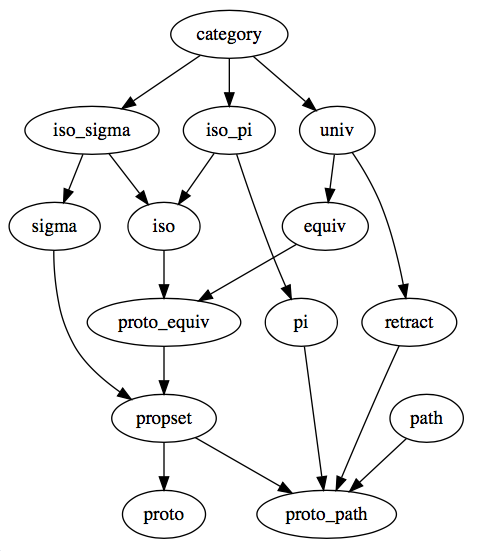
\includegraphics[scale=0.36]{baselib}}
  \caption{Full base library dependencies}
\end{figure}

The amount of code needed for $Nat =_U Fix(Maybe)$ proof is around 400 LOC in modules.

The further development of base library implies:
1) extending run-time facilities;
2) making it useful for building long-running systems and processes;
3) implement the inductive-recursive model for inductive types (development of lambek module).
The main aim is to bring homotopical univalent foundations for run-time systems and models.
Our base library could be used as a first-class mathematical modeling tool or as a sandbox
for developing run-time systems and proving its properties, followed with code extraction
to pure type systems and/or run-time interpreters.

\bibliographystyle{standard}
\bibliography{identity}

\end{document}
